\documentclass[a4paper]{article}
\usepackage[a4paper, margin=1in]{geometry}
% Some basic packages
\usepackage[utf8]{inputenc}
\usepackage[T1]{fontenc}
\usepackage{textcomp}
\usepackage[dutch]{babel}
\usepackage{url}
\usepackage{graphicx}
\usepackage{float}
\usepackage{booktabs}
\usepackage{enumitem}

\pdfminorversion=7

% Don't indent paragraphs, leave some space between them
\usepackage{parskip}

% Hide page number when page is empty
\usepackage{emptypage}
\usepackage{subcaption}
\usepackage{multicol}
\usepackage{xcolor}

% Other font I sometimes use.
% \usepackage{cmbright}

% Math stuff
\usepackage{amsmath, amsfonts, mathtools, amsthm, amssymb}
% Fancy script capitals
\usepackage{mathrsfs}
\usepackage{cancel}
% Bold math
\usepackage{bm}
% Some shortcuts
\newcommand\N{\ensuremath{\mathbb{N}}}
\newcommand\R{\ensuremath{\mathbb{R}}}
\newcommand\Z{\ensuremath{\mathbb{Z}}}
\renewcommand\O{\ensuremath{\emptyset}}
\newcommand\Q{\ensuremath{\mathbb{Q}}}
\newcommand\C{\ensuremath{\mathbb{C}}}

% Easily typeset systems of equations (French package)
\usepackage{systeme}

% Put x \to \infty below \lim
\let\svlim\lim\def\lim{\svlim\limits}

%Make implies and impliedby shorter
\let\implies\Rightarrow
\let\impliedby\Leftarrow
\let\iff\Leftrightarrow
\let\epsilon\varepsilon

% Add \contra symbol to denote contradiction
\usepackage{stmaryrd} % for \lightning
\newcommand\contra{\scalebox{1.5}{$\lightning$}}

% \let\phi\varphi

% Command for short corrections
% Usage: 1+1=\correct{3}{2}

\definecolor{correct}{HTML}{009900}
\newcommand\correct[2]{\ensuremath{\:}{\color{red}{#1}}\ensuremath{\to }{\color{correct}{#2}}\ensuremath{\:}}
\newcommand\green[1]{{\color{correct}{#1}}}

% horizontal rule
\newcommand\hr{
    \noindent\rule[0.5ex]{\linewidth}{0.5pt}
}

% hide parts
\newcommand\hide[1]{}

% si unitx
\usepackage{siunitx}
\sisetup{locale = FR}

% Environments
\makeatother
% For box around Definition, Theorem, \ldots
\usepackage{mdframed}
\mdfsetup{skipabove=1em,skipbelow=0em}
\theoremstyle{definition}
\newmdtheoremenv[nobreak=true]{definitie}{Definitie}
\newmdtheoremenv[nobreak=true]{eigenschap}{Eigenschap}
\newmdtheoremenv[nobreak=true]{gevolg}{Gevolg}
\newmdtheoremenv[nobreak=true]{lemma}{Lemma}
\newmdtheoremenv[nobreak=true]{propositie}{Propositie}
\newmdtheoremenv[nobreak=true]{stelling}{Stelling}
\newmdtheoremenv[nobreak=true]{wet}{Wet}
\newmdtheoremenv[nobreak=true]{postulaat}{Postulaat}
\newmdtheoremenv{conclusie}{Conclusie}
\newmdtheoremenv{toemaatje}{Toemaatje}
\newmdtheoremenv{vermoeden}{Vermoeden}
\newtheorem*{herhaling}{Herhaling}
\newtheorem*{intermezzo}{Intermezzo}
\newtheorem*{notatie}{Notatie}
\newtheorem*{observatie}{Observatie}
\newtheorem*{oef}{Oefening}
\newtheorem*{opmerking}{Opmerking}
\newtheorem*{praktisch}{Praktisch}
\newtheorem*{probleem}{Probleem}
\newtheorem*{terminologie}{Terminologie}
\newtheorem*{toepassing}{Toepassing}
\newtheorem*{uovt}{UOVT}
\newtheorem*{vb}{Voorbeeld}
\newtheorem*{vraag}{Vraag}

\newmdtheoremenv[nobreak=true]{definition}{Definition}
\newtheorem*{eg}{Example}
\newtheorem*{notation}{Notation}
\newtheorem*{previouslyseen}{As previously seen}
\newtheorem*{remark}{Remark}
\newtheorem*{note}{Note}
\newtheorem*{problem}{Problem}
\newtheorem*{observe}{Observe}
\newtheorem*{property}{Property}
\newtheorem*{intuition}{Intuition}
\newmdtheoremenv[nobreak=true]{prop}{Proposition}
\newmdtheoremenv[nobreak=true]{theorem}{Theorem}
\newmdtheoremenv[nobreak=true]{corollary}{Corollary}

% End example and intermezzo environments with a small diamond (just like proof
% environments end with a small square)
\usepackage{etoolbox}
\AtEndEnvironment{vb}{\null\hfill$\diamond$}%
\AtEndEnvironment{intermezzo}{\null\hfill$\diamond$}%
% \AtEndEnvironment{opmerking}{\null\hfill$\diamond$}%

% Fix some spacing
% http://tex.stackexchange.com/questions/22119/how-can-i-change-the-spacing-before-theorems-with-amsthm
\makeatletter
\def\thm@space@setup{%
  \thm@preskip=\parskip \thm@postskip=0pt
}


% Exercise 
% Usage:
% \oefening{5}
% \suboefening{1}
% \suboefening{2}
% \suboefening{3}
% gives
% Oefening 5
%   Oefening 5.1
%   Oefening 5.2
%   Oefening 5.3
\newcommand{\oefening}[1]{%
    \def\@oefening{#1}%
    \subsection*{Oefening #1}
}

\newcommand{\suboefening}[1]{%
    \subsubsection*{Oefening \@oefening.#1}
}


% \lecture starts a new lecture (les in dutch)
%
% Usage:
% \lecture{1}{di 12 feb 2019 16:00}{Inleiding}
%
% This adds a section heading with the number / title of the lecture and a
% margin paragraph with the date.

% I use \dateparts here to hide the year (2019). This way, I can easily parse
% the date of each lecture unambiguously while still having a human-friendly
% short format printed to the pdf.

\usepackage{xifthen}
\def\testdateparts#1{\dateparts#1\relax}
\def\dateparts#1 #2 #3 #4 #5\relax{
    \marginpar{\small\textsf{\mbox{#1 #2 #3 #5}}}
}

\def\@lecture{}%
\newcommand{\lecture}[3]{
    \ifthenelse{\isempty{#3}}{%
        \def\@lecture{Lecture #1}%
    }{%
        \def\@lecture{Lecture #1: #3}%
    }%
    \subsection*{\@lecture}
    \marginpar{\small\textsf{\mbox{#2}}}
}



% These are the fancy headers
\usepackage{fancyhdr}
\pagestyle{fancy}

% LE: left even
% RO: right odd
% CE, CO: center even, center odd
% My name for when I print my lecture notes to use for an open book exam.
% \fancyhead[LE,RO]{Gilles Castel}

\fancyhead[RO,LE]{\@lecture} % Right odd,  Left even
\fancyhead[RE,LO]{}          % Right even, Left odd

\fancyfoot[RO,LE]{\thepage}  % Right odd,  Left even
\fancyfoot[RE,LO]{}          % Right even, Left odd
\fancyfoot[C]{\leftmark}     % Center

\makeatother




% Todonotes and inline notes in fancy boxes
\usepackage{todonotes}
\usepackage{tcolorbox}

% Make boxes breakable
\tcbuselibrary{breakable}

% Verbetering is correction in Dutch
% Usage: 
% \begin{verbetering}
%     Lorem ipsum dolor sit amet, consetetur sadipscing elitr, sed diam nonumy eirmod
%     tempor invidunt ut labore et dolore magna aliquyam erat, sed diam voluptua. At
%     vero eos et accusam et justo duo dolores et ea rebum. Stet clita kasd gubergren,
%     no sea takimata sanctus est Lorem ipsum dolor sit amet.
% \end{verbetering}
\newenvironment{verbetering}{\begin{tcolorbox}[
    arc=0mm,
    colback=white,
    colframe=green!60!black,
    title=Opmerking,
    fonttitle=\sffamily,
    breakable
]}{\end{tcolorbox}}

% Noot is note in Dutch. Same as 'verbetering' but color of box is different
\newenvironment{noot}[1]{\begin{tcolorbox}[
    arc=0mm,
    colback=white,
    colframe=white!60!black,
    title=#1,
    fonttitle=\sffamily,
    breakable
]}{\end{tcolorbox}}




% Figure support as explained in my blog post.
\usepackage{import}
\usepackage{xifthen}
\usepackage{pdfpages}
\usepackage{transparent}
\newcommand{\incfig}[1]{%
    \def\svgwidth{\columnwidth}
    \import{./figures/}{#1.pdf_tex}
}

% Fix some stuff
% %http://tex.stackexchange.com/questions/76273/multiple-pdfs-with-page-group-included-in-a-single-page-warning
\pdfsuppresswarningpagegroup=1

\title{\Huge{Probability 1}}
\author{\huge{Daniel Yu}}
\date{}

\pdfsuppresswarningpagegroup=1

\begin{document}
\maketitle
\newpage% or \cleardoublepage
% \pdfbookmark[<level>]{<title>}{<dest>}
\tableofcontents
\pagebreak
\section{Independence}

\begin{definition}
 Let $\Omega$ be the outcome space and $P$ the probability measure. $A,B \subseteq \Omega$ are events. $A,B$
 are \textbf{independent} if $P[A \cap B] = P[A] \cdot P[B]$. We say $X,Y$ random variables on $\Omega$ are independent
 if $\{X = a\}$ and $\{Y = b\}$ are independent events for every a,b in range of X, Y respectively.   
\end{definition}

\begin{theorem}
  If $\{A_1, \ldots, A_n\} $ is a set of events then for $A \subseteq \{1,\ldots,n\} $:
  \[
    P[\cap_{i \in I} A_i] = \prod_{i \in I} P[A_{i}]
  .\] 
  if the set of events is independent.
\end{theorem}

\begin{definition}
  Define  $P_B$ a new probability measure on  $\Omega$ known as conditional probability.
   \[
     P_B[A] = \frac{P[A\cap B]}{P[B]}
  .\] 
  We can check that this $P_B$ is a probability measure:
   \begin{enumerate}
     \item $P_B [\Omega] = \frac{P[\Omega \cap B}{P[B]} = 1$ 
     \item $P_B[\emptyset] = \frac{P[\emptyset \cap B]}{P[B]} = 0$ 
  \end{enumerate}
  Then independence in terms of this probability measure is defined as:
  \[
    P_B[A] = \frac{P[A \cap B]}{P[A]} = P[A]
  .\]
  You will also see the notation,
  \[
    P[A|B] = \text{ probability of A given B}
  .\] 
\end{definition}

\begin{note}{Example} \\
  $P$ is uniform on  $\{1,2,3,4\} \times \{1,2,3,4\}$. Let $X$ = outcome of first roll. $Y$ = outcome of second roll.
   \[
     P[X = 1] = \{(1,1),(1,2),(1,3),(1,4)\} =\frac{4}{16}=\frac{1}{4}
  .\] 
  The same is true for $P[X=2], \ldots, P[Y=4]$. Thus, $X,Y$ are also both uniform probability measures. And,
  $P[X=a,Y=b] = \frac{1}{16}$ $\forall a,b \in \{1,2,3,4\}$ is a uniform probability measure. Then,
  $P[X=a,Y=b] = P[x=a] \cdot P[y=b] = \frac{1}{4} \cdot \frac{1}{4} = \frac{1}{16}$ and the two rolls
  are independent!
\end{note}

\begin{note}{Example} \\
  Let $M$ be the R.V. representing the maximum of two tosses. Are $M$ and $X$ independent? 
  \[
    P[M=1] = \frac{1}{16}, P[X=1] = \frac{1}{4}
  .\] 
  \[
    P[M=1, X=1] = \frac{1}{16} \neq P[M=1] \cdot P[X=1] = \frac{1}{16} \cdot \frac{1}{4}
  .\] 
  No! Which makes sense!
\end{note}

\begin{note}{Example} \\
  $R = \{ \text{ first roll even} \}$ and $L = \{ \text{ sum of two tolls is 6} \}$ :
  \[
    P[R] = \frac{1}{2}, P[L]=\frac{3}{16}  
  .\] 
  \[
    P[L \cap R] = \frac{2}{16} = \frac{1}{8} \neq P[R] \cdot P[L] = \frac{1}{2} \cdot \frac{3}{16}
  .\] 
  They are not independent.

  However, counterintuitively, when \textbf{L is the set of two rolls whose sum is 5} then the two
  varirables \textbf{are independent}, so this is why we need to prove events are independent.
\end{note}

\begin{remark}
  Independence allows us now to consider \textbf{independent coupling} of distributions which
  allows us to solve the problem of marginals not giving enough information of joint distributions.
\end{remark}

\section{Independent Coupling of Distributions}
I.e. joint distributions with independent variables

\begin{definition}
  When $P[X=x], P[Y=y]$ where  $x,y$ are in the range and  $X,Y$  are independent, we can write the 
  joint probabiltity as:
  \[
    P[X=x, Y=y] = P[X=x] \cdot P[Y=y]
  .\] 
\end{definition}

\begin{definition}
  \textbf{binomial distribution}\\
  Given $P \in [0,1]$ and let  $\left( X_1,X_{2}, \ldots, X_{n} \right)$ to be n independent \textbf{bernoulli}(p)
  random variables. Let $Y = X_1 + X_2 + X_n$, so the $range(Y) = \{0,1,2,\ldots, n\}$. We know that for 
  each bernoulli $\Omega = \{0,1\} $ and for all $n$ independent bernoulli variables:  $\Omega = \{0,1\}^n$
  and $\mid \Omega \mid  = 2^n$. What is the distribution of $Y$?
   \[
     P[Y=0] = P[\{0,0,0,\ldots,0\}] = P[X_1 = 0] + \ldots + P[X_n = 0] = \left( 1-p \right)^n  
  .\] 
  \[
    P[Y=1] = P[\{1,0,\ldots,0\} \cup \{0,1,\ldots,0\} \cup \ldots \cup \{0,0,\ldots,1\}] = 
    n \cdot p \cdot (1-p)^{n-1}
  .\]
  \[
    P[Y=k] = \begin{pmatrix} n \\ k \end{pmatrix} p^k (1-p)^{n-k} 
  .\] 
  where $\begin{pmatrix} n \\ k \end{pmatrix} = \frac{n!}{k! (n-k)!}$ 
  In math terms, we describe $Y \sim binomial(n,p)$ the binomial distribution!
\end{definition}

\begin{definition}{Geometric Distirbution} \\
  Consider the experiment of tossing a coin until $H$ shows up. Let $P[X=H] = p$ where $X$ is a coin toss.
  \[
  \Omega = \{H, TH, TTH, \ldots\} 
  .\] 
  Note that omega is countably infinite, even if you toss a coin a million times you can't be sure there
  will be a heads.

  \[
    P[H] = p
  .\]
  \[
    P[TH] = (1-p)p
  .\] 
  \[
    P[TTH] = (1-p)^2p
  .\] 
  \[
   P[T^n H] = (1-p)^n p
  .\] 
  Let $Z: \Omega \to \R$, the position of $H$ i.e. how many $T$'s. Then  $Z \sim Geo(p)$
\end{definition}


\subsection{Counterintuitive stuff}
\begin{note}{Example}\\
  Let $X,Y$ be two Ber($\frac{1}{2}$) random variables. Let $S= \begin{cases}
    1 \text{ if $X=Y$} \\
    0 \text{ otherwise}
  \end{cases}$ 

  Is $S$ independent of  $X$? Yes! (verify by hand) The same holds for  $S$ and  $Y$!  $S$ is pairwise independent with  $X,Y$.
  However,  $\{X,Y,S\}$ are not jointly independently!!!
  \[
    P[X=1,Y=1,S=0] = 0
  .\] 
  but,
  \[
    P[X=1] \cdot P[Y=1] \cdot P[S=0] = \frac{1}{2} \cdot \frac{1}{2} \cdot \frac{1}{2} \neq 0
  .\] 
  \textbf{pairwise independence does not imply joint independence}
\end{note}

\begin{note}{Example}\\
  Setup an experiment as follows: $X = \{0,1\}$ where $P[X=1]=\frac{1}{2}$.
  \begin{itemize}
    \item If $X=1$, then I toss unfair coin with  $P[H] = \frac{3}{4}$ twice, independently
    \item If $X=0$, then I toss unfair coin with  $P[H] = \frac{1}{4}$ twice, independently
  \end{itemize}
  \[
    \Omega = \{0,1\} \cdot \{H,T\} \cdot \{H,T\}   
  .\] 
  Let's analyze the probabilities
  \[
    P[\{1,H,H\}] = P[X=1, \{H,H\}] = P[\{H,H\} | X=1] \cdot P[X=1] = \frac{9}{32}   
  .\] 
  \[
    P[\{0,H,H\}] =P[X=0, \{H,H\}] = P[\{H,H\} | X=0] \cdot P[X=0] = \frac{1}{32}   
  .\] 
  Then, since the above are disjoint:
  \[
    P[\{H,H\}] = \frac{5}{16} 
  .\] 
  Does $P[\{H,H\}] = P[\text{ first toss H}] \cdot P[\text{ second toss H}]$?
  \[
    P[\text{ first toss H}] = \frac{1}{2} \cdot \frac{3}{4} + \frac{1}{2} \cdot \frac{1}{4} = \frac{1}{2}
  .\] 
  \[
    P[\text{ second toss H}] = \frac{1}{2} \cdot \frac{1}{4} + \frac{1}{2} \cdot \frac{3}{4} = \frac{1}{2}
  .\] 
  \[
    P[\{H,H\}] = \frac{5}{16} \neq \frac{1}{2} \cdot \frac{1}{2} = \frac{1}{4} 
  .\] 
Thus, the "first coin being heads" is NOT independent of the "second coin being heads"!!! Despite
the experiment being clearly defined with the first coin and second coin being tossed independently.

The intuition is that \textbf{information is being passed from the two statements} where if we 
know that the first toss is heads, because the probabilities are weighted to a certain path of 
events to lead to that outcome, this informs us about the probability of the second coin toss 
being heads!!!!
\end{note}

\begin{prop}
  Independent R.V. factor w.r.t to expectations: Let $f(x), g(y)$ be arbitrary functions and  $X,Y$ are R.V.
   \[
     E[f(x) \cdot g(y)] = E[f(x)] \cdot E[g\left( y \right)] 
  .\] 

  \begin{proof}
    \begin{align*}
      E[f(x) \cdot g(y)] &= \sum_{a \in range(x)} \sum_{b \in range(y)} f(a) g(b) P[X=a,Y=b] \\
                         &=  \sum_{a \in range(x)} \sum_{b \in range(y)} f(a) g(b) P[X=a] P[Y=b]\\
                         &=  \sum_{a \in range(x)} f(a) P[X=a] \sum_{b \in range(y)} g(b) P[Y=b]\\ 
                         &= E[f(x)] \cdot E[g(y)]
    .\end{align*}
  \end{proof}
\end{prop}

\begin{corollary}
  If $X,Y$ are independent random variables, they are uncorrelated. Recall that $Cov(X,Y) = E[XY] - E[X] E[Y]$
  and when $Cov(X,Y) = 0$ then they are uncorrelated.
\end{corollary}

\begin{note}{Correlation x= Independence} \\

\begin{figure}[h]
  \centering
  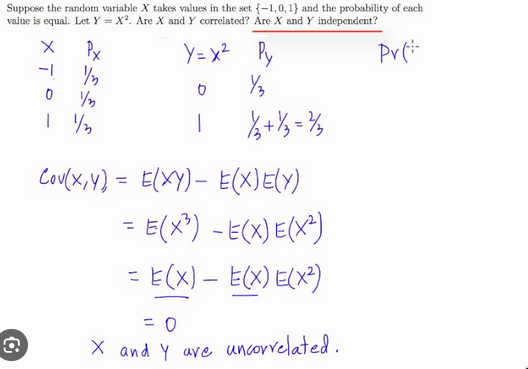
\includegraphics[width=0.8\textwidth]{assets/uncorrelated_not_independent_ex.png}
  \caption{Uncorrelated but Not Independent}
  \label{fig:uncorrelated_not_independent_ex}
\end{figure}
  Finish the analysis at home!
\end{note}

\subsection{Independence for Continuous R.V.}
\begin{definition}
  $X,Y$ are independent if 
   \[
     P[X \leq s, Y \leq t] = P[X \leq s] \cdot P[Y \leq t] \forall s,t
  .\] 
  For cdfs:
  \[
  F_{x,y} (s,t) = F_x(s) - F_x(t)
  .\] 
  Taking partial derivatives, we see the pdfs multiply through:
  \[
  f_{X,Y}(s,t)= f_x(s) \cdot f_Y(t) 
  .\] 
\end{definition}

\begin{definition}
  continuous probability on a continuous space we use pdfs. If $X,Y$ have a joint distribution
  with joint pdf  $f_{X,Y}(s,t)$ :
  \[
    P[Y=t, X=s] = \frac{P[Y=t,X=s]}{P[X=s]}
  .\] 
  As the marginal pdf of $X$:
  \[
    \int_{-\infty}^{\infty} f_{X,Y}(s,t) = \text{ marginal pdf of X} f_X(s)  
  .\] 
  pdf of $Y$ given  $X=s$:
   \[
  f_{Y|X=s} (t) = \frac{f_{X,Y}(s,t)}{\int_{-\infty}^{\infty} f_{X,Y} (s,t) dt}
  .\] 
\end{definition}


\end{document}
